%%This is a very basic article template.
%%There is just one section and two subsections.
\documentclass[a4paper, 11pt]{article}
\usepackage[ngerman]{babel}
\usepackage[T1]{fontenc}
\usepackage[utf8]{inputenc} 
\usepackage{amsthm,amsfonts,amssymb,amsmath,amsbsy}
\usepackage{ngerman}
\usepackage{hyperref}
\usepackage{amsthm}
\usepackage{graphicx}
\usepackage{listings}

\pagestyle{empty}
\author{Sarah Lutteropp, Parto Karwat}
\title{Basispraktikum Hardwarenaher Systementwurf WS 11/12 \\ Arbeitsbericht 1}
\date{\today}

\theoremstyle{definition}
\newtheorem{definition}{Definition}
\theoremstyle{plain}
\newtheorem{satz}{Satz}

\begin{document}

\maketitle

\section{Vorwort}
In diesem Aufgabenblatt ging es darum, einfache Schaltungen in VHDL zu beschreiben und zu testen, um mit der Sprache VHDL und den Simulationswerkzeugen (Modelsim, GHDL, GTKWave) vertraut zu werden.

\section{Schaltungsentwurf mit VHDL}

\subsection{Allgemeine Vorgehensweise}
Die VHDL-Dateien haben wir mithilfe des Texteditors Kate erstellt und bearbeitet. Besonders am Anfang hatten wir parallel zum Editorfenster die Folien der VHDL-Einführung geöffnet und uns von den Codebeispielen auf den Folien bei der Entwicklung unseres eigenen Quellcodes leiten lassen. Beim Coden haben wir uns alle paar Zeilen abgewechselt und simultan den Quelltext besprochen.

\subsection{1.1 bis 1.4}
Siehe angehängte Quelltexte.

\subsection{Bonusaufgabe}
Als Schaltung unserer Wahl haben wir eine Schaltung mit drei Eingängen und einem Ausgang implementiert, die folgendes leistet: Die Schaltung zählt einen Wert modulo 42 hoch und gibt ihn aus. Dabei haben die drei Eingänge folgende Funktion: Der erste Eingang dient dazu, die clk weiterzugeben, der zweite Eingang fungiert als Reset-Eingang und der dritte Eingang signalisiert, dass das Modul das Hochzählen pausieren soll. Ist der Reset-Eingang auf 0 gelegt, so gibt die Schaltung eine 0 aus. Ist dieser auf 1 gelegt, so zählt die Schaltung, falls sie gerade nicht pausieren soll, modulo 42 hoch.
Hierzu haben wir folgende weitere Bibliothek (nach einer Internetrecherche) eingebunden: ieee.numeric\_std.all .
Diese Bibliothek stellt u.a. Funktionalitäten zur Umwandlung eines Integer-Wertes in einen std\_logic\_vector 
zur Verfügung. 
\newline
Die Bonusaufgabe ist in den Dateien bonus.vhd und bonus\_tb.vhd gespeichert.

\section{Simulation}

\subsection{Modelsim}

\subsubsection{Direktes Setzen der Eingänge}
Geht mit `force', z.B.:
\begin{lstlisting}
force -freeze sim:/in2_out1/a 0
\end{lstlisting}

\subsubsection{Simulation mit Hilfe einer Testbench}
Hier ein Ausschnitt aus der Simulation der Bonusaufgabe: \newline
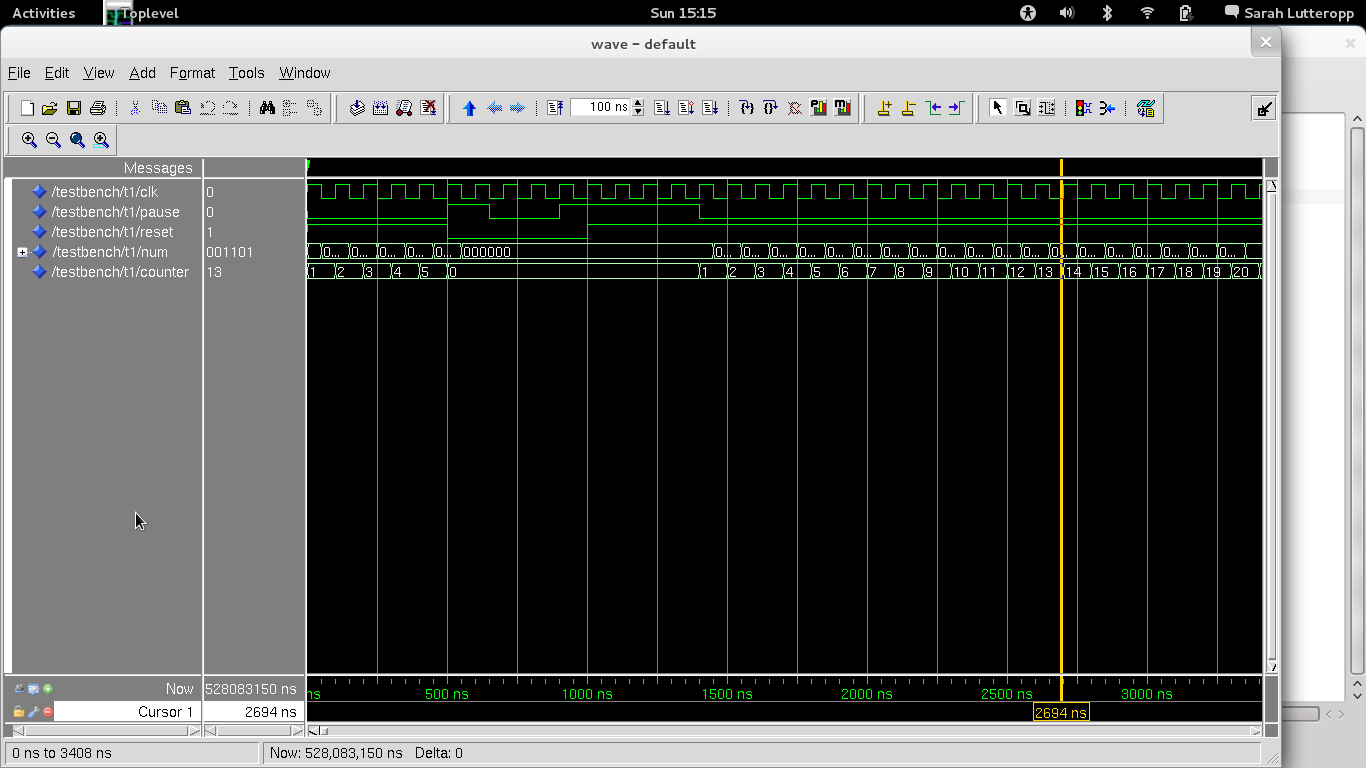
\includegraphics[width=\textwidth]{bonus.png}

\subsubsection{Skriptgesteuerte Ausführung}
vsim -c -do script.do \newline
Ein Beispielskript ist unter dem Dateinamen script.do zu finden. \newline
... (hier sollten wir noch was hinzufügen)

\subsection{GHDL und GTKWave}
Um unsere Testbenches zu simulieren, haben wir folgende Befehle verwendet:
\begin{lstlisting}
$ ghdl -i *.vhd \newline
$ ghdl -m NAME_DER_TESTBENCH
$ ghdl -r NAME_DER_TESTBENCH --wave=design.ghw --stop-time=2000ns
$ gtkwave design.ghw
\end{lstlisting}

Hier ein Beispiel für den Signalverlauf der zum Modul mynand zugehörigen Testbench bei GTKWave:
\newline
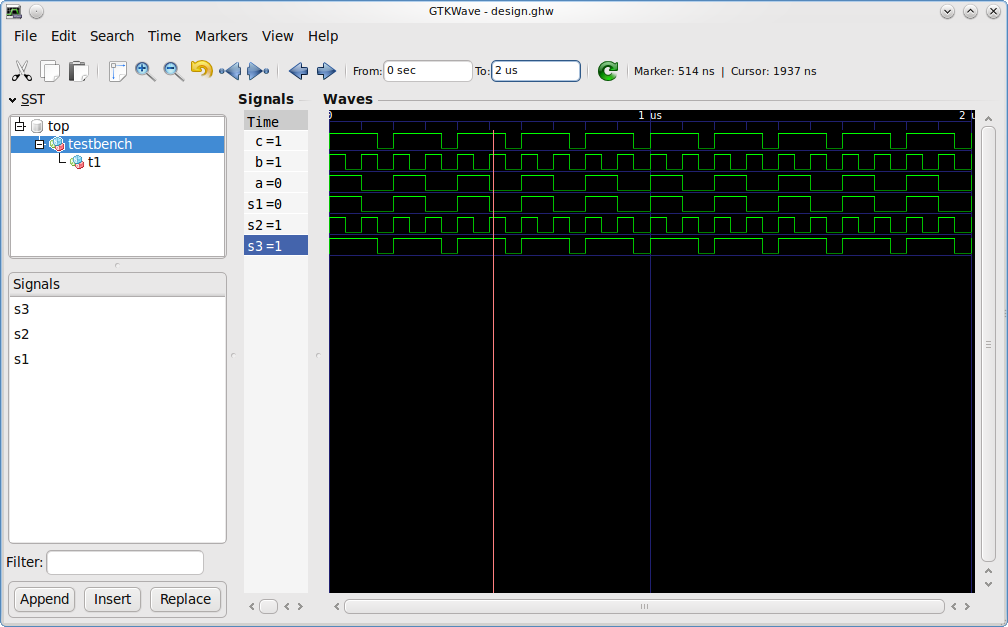
\includegraphics[width = 1\textwidth]{gtkwave_mynand.png}

\subsection{Vor- und Nachteile der verschiedenen Simulationsprogramme}

\subsubsection{Modelsim}

\begin{tabular}{p{7cm}|p{7cm}}
\textbf{Vorteile} & \textbf{Nachteile} \\
\hline 
$\bullet$ direktes Setzen der Eingänge möglich & $\bullet$ unpraktischer eingebauter Texteditor \\
$\bullet$ reichlich Dokumentation vorhanden & $\bullet$ erfordert Nutzungslizenz \\
$\bullet$ hoher Bekanntheitsgrad & $\bullet$ kostenpflichtig, closed source \\
$\bullet$ alles in einer Anwendung & $\bullet$ leicht gewöhnungsbedürftige Bedienung zu Anfang \\
$\bullet$ große Funktionsvielfalt & $\bullet$ mühsamere Installation
\end{tabular}

\subsubsection{GHDL}

\begin{tabular}{p{7cm}|p{7cm}}
\textbf{Vorteile} & \textbf{Nachteile} \\
\hline 
$\bullet$ einfache Bedienung per Kommandozeile & $\bullet$ Bedienung nur über Kommandozeile \\
$\bullet$ kostenfrei, Open Source & $\bullet$ weniger Dokumentation vorhanden \\
$\bullet$ statisches Verhalten, keine Eingriffsmöglichkeit & $\bullet$ erfordert Testbenches \\
$\bullet$ andere Fehlermeldungen als Modelsim & $\bullet$ benötigt Configurations, falls mehrere Testbenches in einer Entity testbench enthalten sind
\end{tabular}

\subsubsection{GTKWave}

\begin{tabular}{p{7cm}|p{7cm}}
\textbf{Vorteile} & \textbf{Nachteile} \\
\hline 
$\bullet$ GUI vorhanden & $\bullet$ weniger Einstellungsmöglichkeiten \\
$\bullet$ kostenfrei, Open Source & $\bullet$ weniger Dokumentation vorhanden \\
$\bullet$ übersichtliche Anzeige & $\bullet$ keine Möglichkeit, manuell Signale zu setzen und in die Simulation einzugreifen \\
$\bullet$  selbsterklärend & $\bullet$ nur reiner Viewer von von GHDL vorher generierter Datei \\
 & $\bullet$ `Zoom best fit' nicht automatisch eingestellt
\end{tabular}

\end{document}